% GNUPLOT: LaTeX picture with Postscript
\begingroup
  \makeatletter
  \providecommand\color[2][]{%
    \GenericError{(gnuplot) \space\space\space\@spaces}{%
      Package color not loaded in conjunction with
      terminal option `colourtext'%
    }{See the gnuplot documentation for explanation.%
    }{Either use 'blacktext' in gnuplot or load the package
      color.sty in LaTeX.}%
    \renewcommand\color[2][]{}%
  }%
  \providecommand\includegraphics[2][]{%
    \GenericError{(gnuplot) \space\space\space\@spaces}{%
      Package graphicx or graphics not loaded%
    }{See the gnuplot documentation for explanation.%
    }{The gnuplot epslatex terminal needs graphicx.sty or graphics.sty.}%
    \renewcommand\includegraphics[2][]{}%
  }%
  \providecommand\rotatebox[2]{#2}%
  \@ifundefined{ifGPcolor}{%
    \newif\ifGPcolor
    \GPcolortrue
  }{}%
  \@ifundefined{ifGPblacktext}{%
    \newif\ifGPblacktext
    \GPblacktexttrue
  }{}%
  % define a \g@addto@macro without @ in the name:
  \let\gplgaddtomacro\g@addto@macro
  % define empty templates for all commands taking text:
  \gdef\gplbacktext{}%
  \gdef\gplfronttext{}%
  \makeatother
  \ifGPblacktext
    % no textcolor at all
    \def\colorrgb#1{}%
    \def\colorgray#1{}%
  \else
    % gray or color?
    \ifGPcolor
      \def\colorrgb#1{\color[rgb]{#1}}%
      \def\colorgray#1{\color[gray]{#1}}%
      \expandafter\def\csname LTw\endcsname{\color{white}}%
      \expandafter\def\csname LTb\endcsname{\color{black}}%
      \expandafter\def\csname LTa\endcsname{\color{black}}%
      \expandafter\def\csname LT0\endcsname{\color[rgb]{1,0,0}}%
      \expandafter\def\csname LT1\endcsname{\color[rgb]{0,1,0}}%
      \expandafter\def\csname LT2\endcsname{\color[rgb]{0,0,1}}%
      \expandafter\def\csname LT3\endcsname{\color[rgb]{1,0,1}}%
      \expandafter\def\csname LT4\endcsname{\color[rgb]{0,1,1}}%
      \expandafter\def\csname LT5\endcsname{\color[rgb]{1,1,0}}%
      \expandafter\def\csname LT6\endcsname{\color[rgb]{0,0,0}}%
      \expandafter\def\csname LT7\endcsname{\color[rgb]{1,0.3,0}}%
      \expandafter\def\csname LT8\endcsname{\color[rgb]{0.5,0.5,0.5}}%
    \else
      % gray
      \def\colorrgb#1{\color{black}}%
      \def\colorgray#1{\color[gray]{#1}}%
      \expandafter\def\csname LTw\endcsname{\color{white}}%
      \expandafter\def\csname LTb\endcsname{\color{black}}%
      \expandafter\def\csname LTa\endcsname{\color{black}}%
      \expandafter\def\csname LT0\endcsname{\color{black}}%
      \expandafter\def\csname LT1\endcsname{\color{black}}%
      \expandafter\def\csname LT2\endcsname{\color{black}}%
      \expandafter\def\csname LT3\endcsname{\color{black}}%
      \expandafter\def\csname LT4\endcsname{\color{black}}%
      \expandafter\def\csname LT5\endcsname{\color{black}}%
      \expandafter\def\csname LT6\endcsname{\color{black}}%
      \expandafter\def\csname LT7\endcsname{\color{black}}%
      \expandafter\def\csname LT8\endcsname{\color{black}}%
    \fi
  \fi
    \setlength{\unitlength}{0.0500bp}%
    \ifx\gptboxheight\undefined%
      \newlength{\gptboxheight}%
      \newlength{\gptboxwidth}%
      \newsavebox{\gptboxtext}%
    \fi%
    \setlength{\fboxrule}{0.5pt}%
    \setlength{\fboxsep}{1pt}%
\begin{picture}(10800.00,7560.00)%
    \gplgaddtomacro\gplbacktext{%
      \csname LTb\endcsname%%
      \put(870,680){\makebox(0,0)[r]{\strut{}-0.3}}%
      \csname LTb\endcsname%%
      \put(870,1300){\makebox(0,0)[r]{\strut{}-0.2}}%
      \csname LTb\endcsname%%
      \put(870,1920){\makebox(0,0)[r]{\strut{}-0.1}}%
      \csname LTb\endcsname%%
      \put(870,2540){\makebox(0,0)[r]{\strut{}0}}%
      \csname LTb\endcsname%%
      \put(870,3160){\makebox(0,0)[r]{\strut{}0.1}}%
      \csname LTb\endcsname%%
      \put(972,494){\makebox(0,0){\strut{}-1.00$\pi$}}%
      \csname LTb\endcsname%%
      \put(1934,494){\makebox(0,0){\strut{}-0.80$\pi$}}%
      \csname LTb\endcsname%%
      \put(2897,494){\makebox(0,0){\strut{}-0.60$\pi$}}%
      \csname LTb\endcsname%%
      \put(3859,494){\makebox(0,0){\strut{}-0.40$\pi$}}%
      \csname LTb\endcsname%%
      \put(4821,494){\makebox(0,0){\strut{}-0.20$\pi$}}%
      \csname LTb\endcsname%%
      \put(5784,494){\makebox(0,0){\strut{}0.00$\pi$}}%
      \csname LTb\endcsname%%
      \put(6746,494){\makebox(0,0){\strut{}0.20$\pi$}}%
      \csname LTb\endcsname%%
      \put(7708,494){\makebox(0,0){\strut{}0.40$\pi$}}%
      \csname LTb\endcsname%%
      \put(8670,494){\makebox(0,0){\strut{}0.60$\pi$}}%
      \csname LTb\endcsname%%
      \put(9633,494){\makebox(0,0){\strut{}0.80$\pi$}}%
      \csname LTb\endcsname%%
      \put(10595,494){\makebox(0,0){\strut{}1.00$\pi$}}%
    }%
    \gplgaddtomacro\gplfronttext{%
      \csname LTb\endcsname%%
      \put(276,2230){\rotatebox{-270}{\makebox(0,0){\strut{}$\Delta \chi^2 - \Delta \chi^2_0$}}}%
      \csname LTb\endcsname%%
      \put(5783,215){\makebox(0,0){\strut{}$\delta_\text{CP}$}}%
      \csname LTb\endcsname%%
      \put(3939,3377){\makebox(0,0){\strut{}Difference}}%
      \csname LTb\endcsname%%
      \put(3758,3191){\makebox(0,0)[l]{\strut{}11a}}%
      \csname LTb\endcsname%%
      \put(3758,3005){\makebox(0,0)[l]{\strut{}11b}}%
      \csname LTb\endcsname%%
      \put(3758,2819){\makebox(0,0)[l]{\strut{}8}}%
    }%
    \gplgaddtomacro\gplbacktext{%
      \csname LTb\endcsname%%
      \put(870,3780){\makebox(0,0)[r]{\strut{}0}}%
      \csname LTb\endcsname%%
      \put(870,4702){\makebox(0,0)[r]{\strut{}50}}%
      \csname LTb\endcsname%%
      \put(870,5623){\makebox(0,0)[r]{\strut{}100}}%
      \csname LTb\endcsname%%
      \put(870,6545){\makebox(0,0)[r]{\strut{}150}}%
      \csname LTb\endcsname%%
      \put(870,7466){\makebox(0,0)[r]{\strut{}200}}%
      \csname LTb\endcsname%%
      \put(972,3594){\makebox(0,0){\strut{}}}%
      \csname LTb\endcsname%%
      \put(1934,3594){\makebox(0,0){\strut{}}}%
      \csname LTb\endcsname%%
      \put(2897,3594){\makebox(0,0){\strut{}}}%
      \csname LTb\endcsname%%
      \put(3859,3594){\makebox(0,0){\strut{}}}%
      \csname LTb\endcsname%%
      \put(4821,3594){\makebox(0,0){\strut{}}}%
      \csname LTb\endcsname%%
      \put(5784,3594){\makebox(0,0){\strut{}}}%
      \csname LTb\endcsname%%
      \put(6746,3594){\makebox(0,0){\strut{}}}%
      \csname LTb\endcsname%%
      \put(7708,3594){\makebox(0,0){\strut{}}}%
      \csname LTb\endcsname%%
      \put(8670,3594){\makebox(0,0){\strut{}}}%
      \csname LTb\endcsname%%
      \put(9633,3594){\makebox(0,0){\strut{}}}%
      \csname LTb\endcsname%%
      \put(10595,3594){\makebox(0,0){\strut{}}}%
    }%
    \gplgaddtomacro\gplfronttext{%
      \csname LTb\endcsname%%
      \put(378,5623){\rotatebox{-270}{\makebox(0,0){\strut{}$\Delta \chi^2$}}}%
      \csname LTb\endcsname%%
      \put(5783,3538){\makebox(0,0){\strut{}}}%
      \csname LTb\endcsname%%
      \put(3721,7004){\makebox(0,0){\strut{}}}%
      \csname LTb\endcsname%%
      \put(3758,7004){\makebox(0,0)[l]{\strut{}0}}%
      \csname LTb\endcsname%%
      \put(3758,6818){\makebox(0,0)[l]{\strut{}11a}}%
      \csname LTb\endcsname%%
      \put(3758,6632){\makebox(0,0)[l]{\strut{}11b}}%
      \csname LTb\endcsname%%
      \put(3758,6446){\makebox(0,0)[l]{\strut{}8}}%
    }%
    \gplbacktext
    \put(0,0){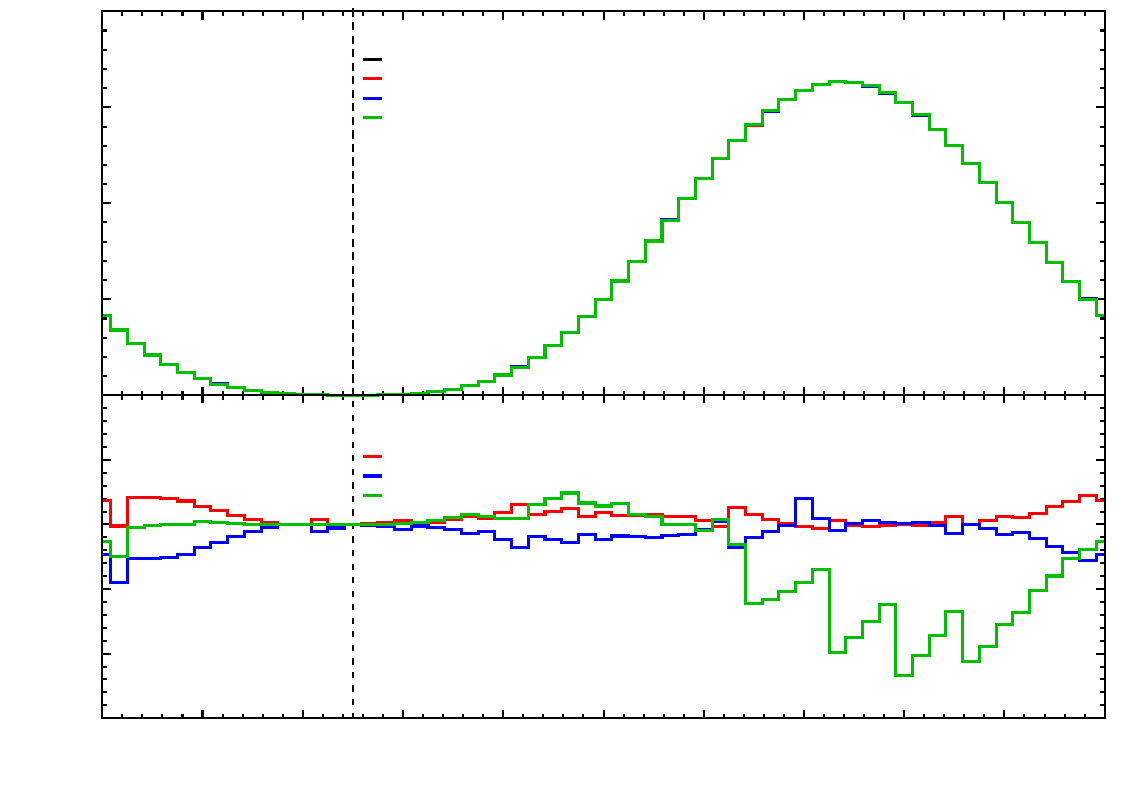
\includegraphics{pics/0_11a_11b_8_chi2_dCP}}%
    \gplfronttext
  \end{picture}%
\endgroup
